\documentclass[11pt, letterpaper]{article}
\usepackage[backend=bibtex]{biblatex}
\bibliography{bib}
\usepackage[utf8]{inputenc}
\usepackage{amsmath}
\usepackage{amsfonts}
\usepackage{amssymb}
\usepackage{fullpage}
\usepackage{lmodern}
\usepackage{graphicx}
\usepackage{gensymb}
\usepackage{parskip}
\author{Revan~Sopher}
\title{Detecting Planes in Real-Time for Camera Display Communications\\
{\large Independent Study Report}}
\begin{document}
\maketitle

\begin{abstract}
TODO
\end{abstract}

\section{Introduction}

\subsection{Visual MIMO}
The aim of the Visual MIMO project thus far has been to embed messages within images by varying the intensity of patches of the image, and to reliably extract these messages from pictures of the image displayed on a screen.

The existing software system is capable of detecting the computer monitor, in order to to consider only the displayed image, but encounters difficulties with the variance in photometry dependent on camera and display type, and the spatial positioning of the two.
This is addressed via radiometric calibration: nearly invisible patches are created on the corners of the image using histogram equalization, creating calibration data.

TODO: expand

\subsection{Mobile Challenges}
Although the Visual MIMO project is intended to make use of the ubiquity of handheld cameras, previous work has been reliant on a precise, static configuration of high quality SLR camera and a desktop computer.
The purpose of this independent study will be to facilitate the implementation of this algorithm to run on a mobile device, such as a smartphone or Google Glass.
This will require special considerations and optimizations to compensate for the significantly weaker processor and average cameras: the processing limitations can be mitigated by lower level programming and memory management using the Android Native Development Kit, but the lower quality image and light sensors may need experimentation.

The primary focus of this study is in addressing the issues that arise from the spatial differences between the camera and the screen: although radiometric calibration can mitigate such differences, the resulting calibration is only valid for the current positions, resulting in a fragile setup unsuitable for casual demonstrations.

The goal is to increase the accuracy of imperfect positioning, without requiring explicit calibration.

\section{Image Tracking with Vuforia}
The Android application is built around the Qualcomm Vuforia SDK \cite{vuforia}, a library meant for facilitating the construction of Augmented Reality applications.
Vuforia is used for its image tracking capabilities: known "targets" are trained ahead of time, and are quickly and reliably detected in realtime.

Upon detection,	Vuforia provides the pose matrix. Combined with the known size of the target image, we can calculate the position of the image corners.

\section{Native Image Processing}
\subsection{Image Format}
The camera image is encoded in RGB888, meaning a one dimensional array of tuples of red, grean, blue values from 0 to 255.
This format was selected over alternatives for its large information quantity.

\subsection{Skew Correction}
The usage of a mobile device for image capture necessarily forecloses angular calibration.
As such, the image captured is usually not head on (Figure~\ref{fig:skew}).
In this step, we use a projective transformation to correct for skew.

First we obtain the $3 \times 3$ transformation matrix, such that:

$$
\begin{pmatrix}
t_i x_i^*\\
t_i y_i^*\\
t_i
\end{pmatrix}\\
= \text{transformation\_matrix} \cdot
\begin{pmatrix}
t_i x_i\\
t_i y_i\\
1
\end{pmatrix}
$$
That is, we map each corner to the proper rectangular positions.

Having calculated the corner positions previously and knowing the shape of the original image, this is easily accomplished with OpenCV\cite{opencv_getperspectivetransform}.

Next, we apply the transformation by multiplying the found matrix with each point in the image.
This is again straightforward with OpenCV \cite{opencv_warpperspective}, yielding Figure~\ref{fig:skew2}.

\begin{figure}[hbtp]
\centering
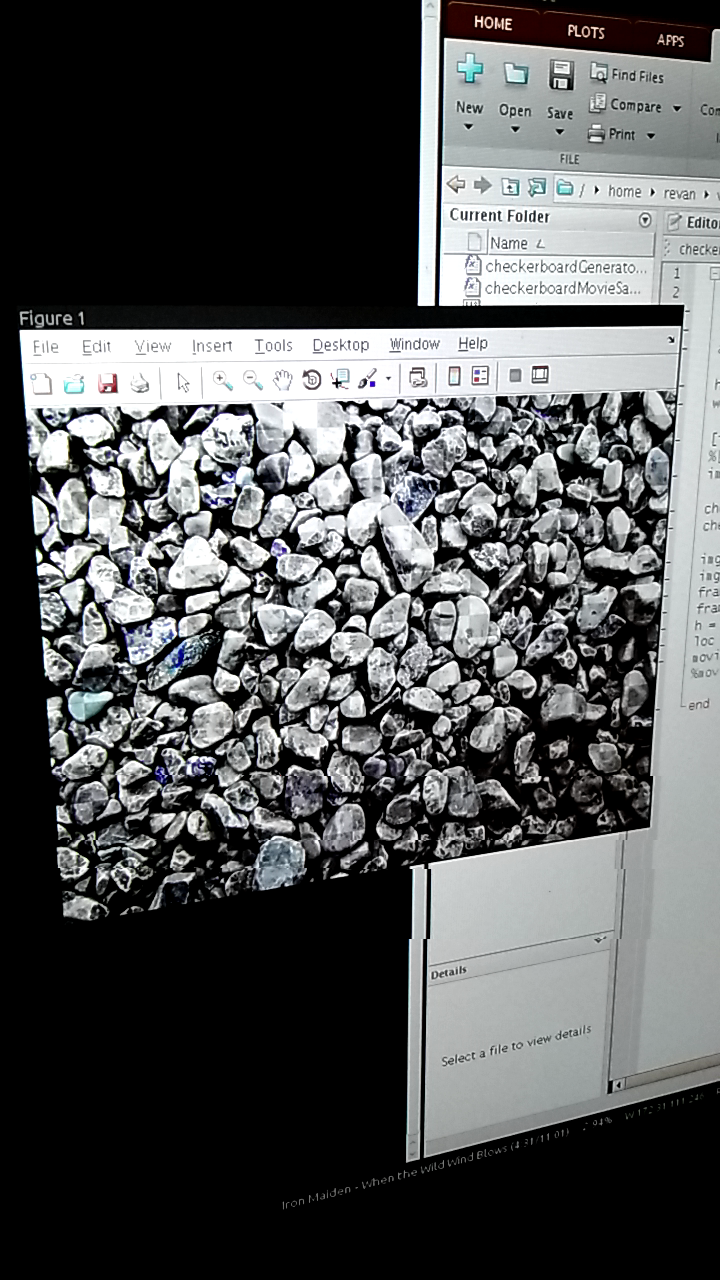
\includegraphics[scale=0.10]{img/skew.png}
\caption{An image viewed at an oblique angle.}
\label{fig:skew}
\end{figure}

\begin{figure}[hbtp]
\centering
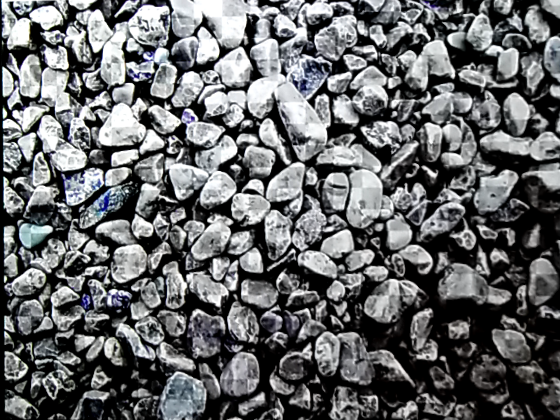
\includegraphics[scale=0.2]{img/skew2.png}
\caption{The image, skew-corrected by projective transformation.}
\label{fig:skew2}
\end{figure}

\subsection{Histogram Equalization}
TODO (once I work out partial histogram equalization)

\subsection{Subtraction}
With both targets skew-adjusted and normalized, we subtract one image from the other:

$$\text{dst}[I] = \text{saturate}(\text{src1}[I] - \text{src2}[I])$$ where $I$ is the image matrix\cite{opencv_subtraction}.

As the non-message part of the images should match up, this should leave only the message (Figure~\ref{fig:subtract}).

\begin{figure}[hbtp]
\centering
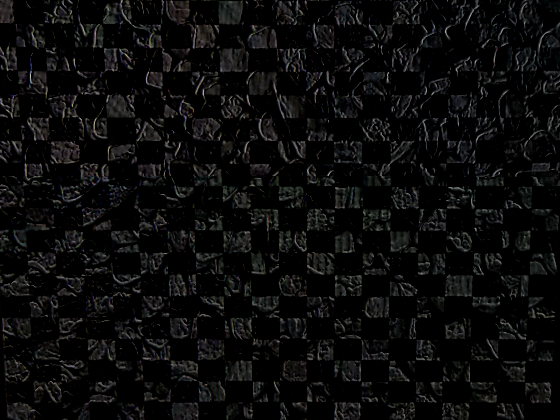
\includegraphics[scale=0.2]{img/subtract.png}
\caption{An example of subtraction.}
\label{fig:subtract}
\end{figure}

\subsection{Information Extraction}
Having isolated the encoded pattern, we must then decode the information inside.

TODO

\section{Google Glass}
TODO: future work?

\section{Future Work}
TODO

\printbibliography
\end{document}
